Despite the delays in timeline, the management of the project has been satisfactory. Meetings with the project supervisor have occurred every week and have proven to be very effective. The meetings have mostly consisted on reviewing the Kanban board of the project, exemplified in Figure \ref{fig:trello-kanban}. Created using the Trello\cite{trello} website, it divides the project tasks in three categories: ``To do'', ``In progress'' and ``Done''. This has allowed the project supervisor to be receive frequent updates regarding the progress, resulting in a more efficient usage of the time dedicated to meetings.

\begin{figure}[h]
    \centering
    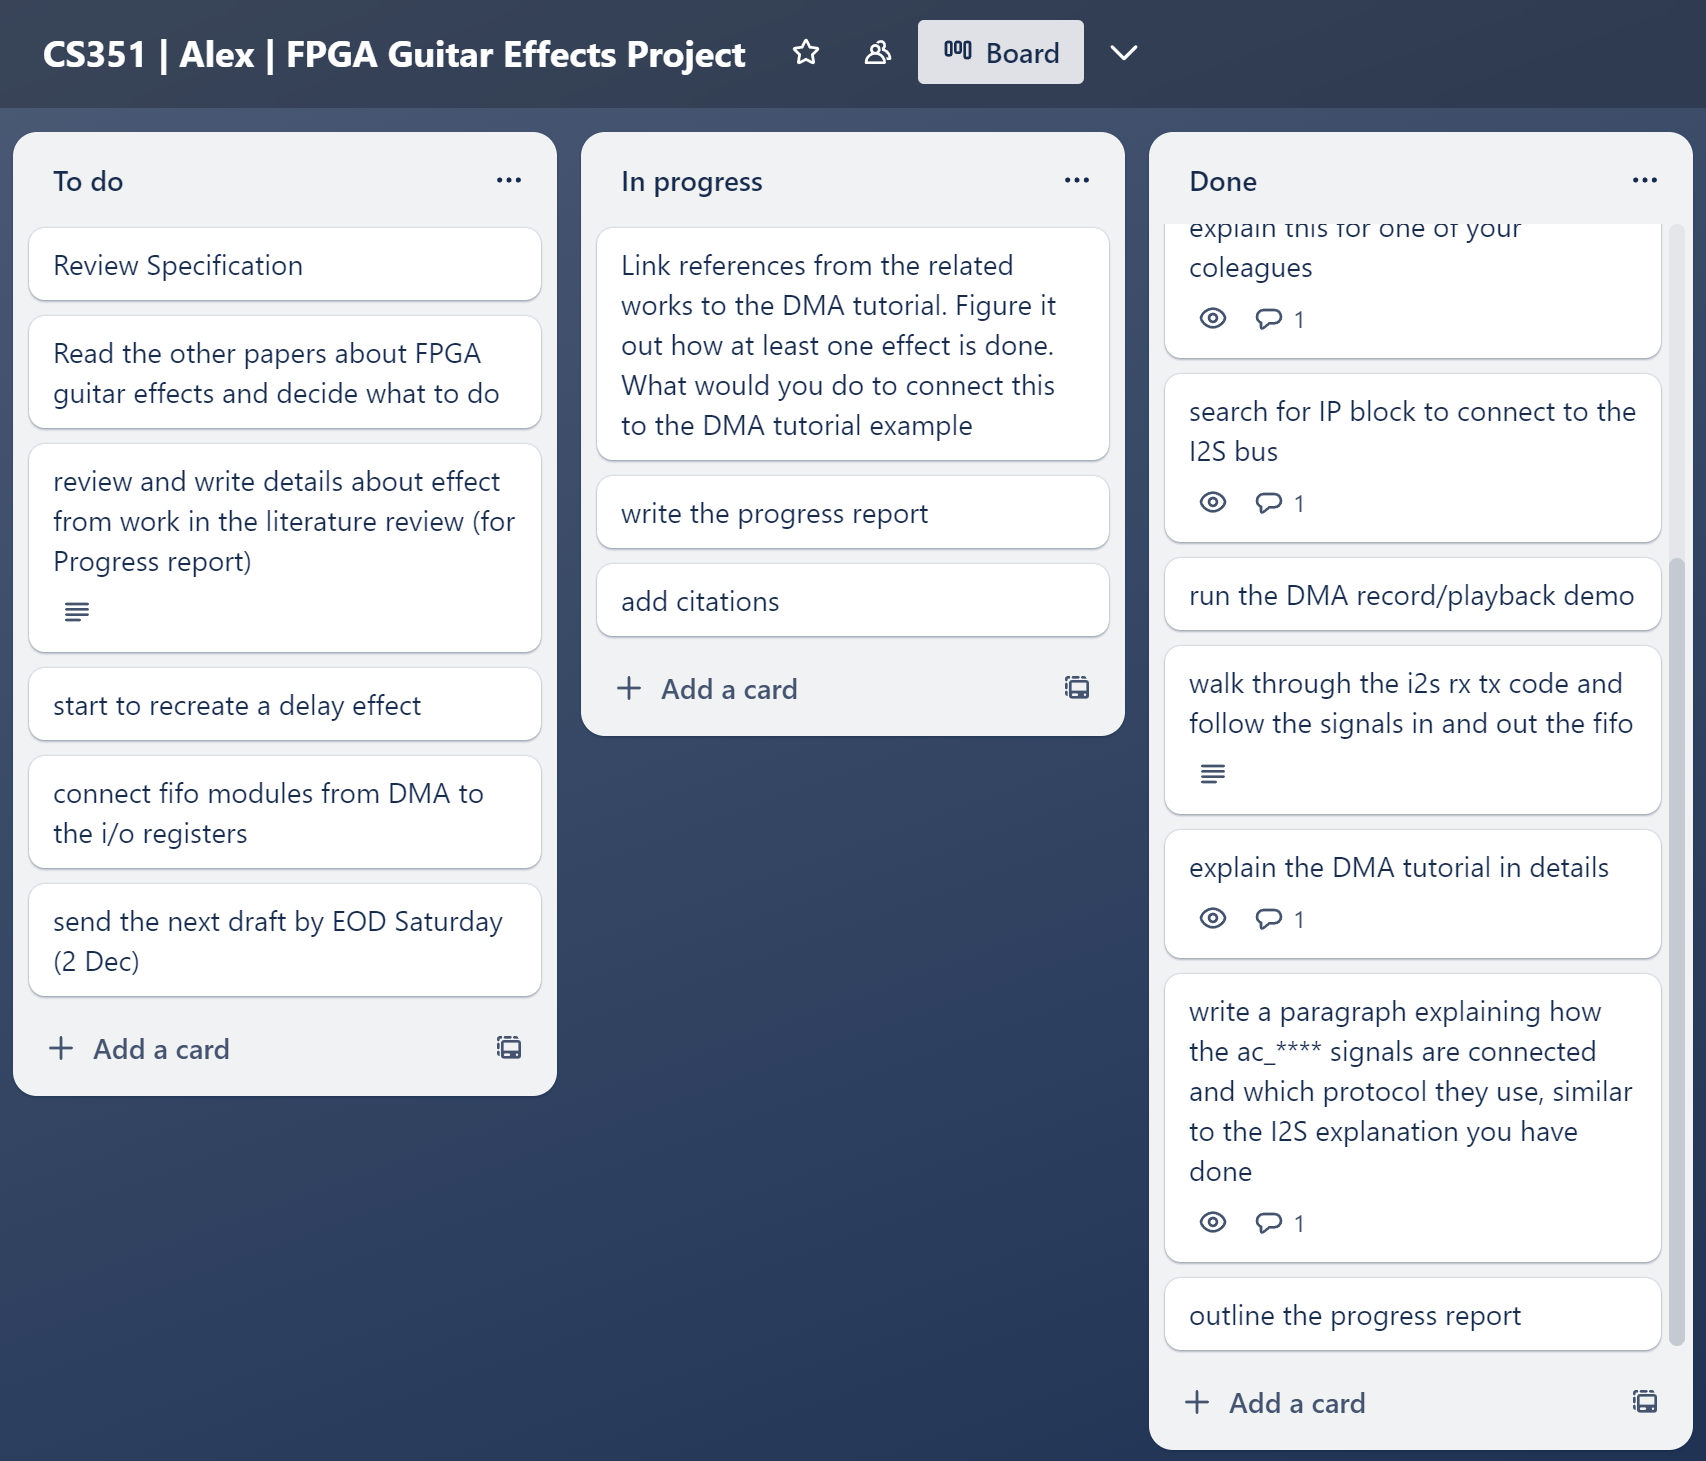
\includegraphics[width=0.9\linewidth]{progress-report/kanban.png}
    \caption{Planning Tasks with a Kanban Board on Trello}
    \label{fig:trello-kanban}
\end{figure}

Moreover, the meetings have also represented a time to reflect on future approaches or discuss any issues that were encountered over the previous week. 

Another remark about the effectiveness of the project management is the avoidance of any substantial progress loss as a result of the experienced hardware failure. The analysis of risks and the continuous usage of cloud storage and version control software (GitHub\cite{github}) as a method of prevention has saved the project from a potential severe complication.